\chapter{Naturally Parameterized NLP framework}

%%%%%%%%%%%%%%%%%%% SECTION 1 %%%%%%%%%%%%%%%%%%%%%%%%%%%%%
\section{Introduction}\label{CH4S1}
%%%%%%%%%%%%%%%%%%%%%%%%%%%%%%%%%%%%%%%%%%%%%%%%%%%%%%%%%%%
This chapter presents a parametric nonlinear programming (\acrshort{pnlp}) 
framework
that extends the problem solving capabilites of the Hybrid \acrshort{nlp} beam 
element beyond analyses concerned with mechanical loading. Such cases can be 
contact problems or structural sensitivity analysis. A strong feature of this 
framework lies in the utlizitation of homotopy continuation principles
in order to establish conditions of global
convergence to at least one solution. With the term ``solution" we broadly 
refer to any critical point for the objective function, which in the present 
context is the \acrshort{tpe}, with respect to the system variables. 

Homotopy continuation, which forms the backbone of the PNLP framework, has been 
the subject of extensive studies in the field of applied 
mathematics\cite{Allgower:2003,Rheinboldt:2000,Keller:1978,Li:1980,Chow:1978,Chow:1979,
Watson:1989,Watson:1990,Allgower:1981,Rheinboldt:1980,Rheinboldt:1983,Wayburn:1987}
as a technique for ``globalizing" root finding 
algorithms. That is, even if the initial guess is not in the neighborhood of a 
root, homotopy theory guarantees convergence to at least one root, given 
certain regularity conditions hold. These conditions in essence establish the 
existence of a smooth path connecting the initial guess and that root.  When 
applied to finding a root of a system of equations $F(x)=0$, this can be done 
by introducing an ``easy" problem whose a solution is easy to find, say 
$x-x_0=$, and then construct a homotopy function $H(x,t) = tF(x)+(1-t)(x-x_0)$, 
which represents a system of $n$ equations with $n+1$ unknowns. The system  
$H(x,t)=0$ is sequantially solved for a discretization of $t\in[0,1]$, starting 
at $t_0=0$, where the solution is known (``initial guess"). When $t=1$ we have 
arrived at a root of the initial problem $F(x)=0$. The process of varying $t$ 
from 0 to 1 and solving the homotopy function is called deformation (not to be 
confused with mechanical deformation) and construction of such a homotopy 
function is called artificial homotopy.  It is clear that the same principles 
can be applied if system $F(x)=0$ is undetermined, with $n$ equations, $n+1$ 
unknowns and a solution is available or can be found easily. In a nonlinear 
optimization context, application of the same principles have led to the 
formulation of global optimization 
algorithms\cite{Kojima:1984,Gfrerer:1985,Guddat:1990,Gfrerer:1983,Zangwill:1981,Poore:1990,
Jongen:1990,Tiahrt:1989}. In addition, this 
framework highlights the firm theoretical
underpinnings of various incremental methods that
have been developed independently over the past decades for the numerical 
treatment 
of engineering 
problems\cite{Crisfield3,Wempner:1971,Bergan:1978,Bergan:1978b,Batoz:1979,Riks:1979,
Ramm:1981,Watson:1985,Sideris:2017,Byrne:1985,Ushida:1984,Borkovsky:2010,Besanko:2010,
Herings:2010,Bartovn:2016,Barendrecht:2018}. Application of this framework for 
approximating roots 
of systems of equations is commonly referred to as numerical continuation, 
whereas in the the context of finding optimizers it is termed parametric 
optimization or \acrshort{pnlp}.
  
In structural mechanics, differential equilibrium equations can be reformulated 
as an optimization problem due to the existence of a variational structure, as 
discussed in Chapter \ref{chapter:CH2}. Thus, the \acrshort{pnlp} framework 
provides a suitable and versatile engine for generating global solutions to 
engineering problems using the Hybrid 
\acrshort{nlp}-based element, since it allows for the incorporation of 
constraint
specifications directly at the minimization statement. It is shown that, in the 
presence of inequality constraints, the global path that connects the initial 
guess to a critical point is continuous but piecewise 
differentiable\cite{Kojima:1984,Guddat:1990,Gfrerer:1985}. Finally, utilizing 
the underlying 
homotopy arguments, we establish the conditions under which the path we follow 
is unique and convergent to at least one critical point. Non-uniqueness of the 
homotopy path implies the existence of bifurcation points. Because the 
derivations do not make use of artificial functions in order to introduce 
initial guesses, we termed the formulation as Naturally Parameterized NLP 
(\acrshort{npnlp}). While this has the downside of requiring a known solution 
of the system in order to initiate the homotopy deformation process, in 
structural mechanics such states can often be found easily (e.g. initial 
configuration).

This chapter is divided into 5 sections. In the first section we give an 
overview of homotopy continuation as applied in (globally) solving systems of 
nonlinear equations and in parametric optimization. In the second section 
formulate the \acrshort{npnlp} framework for the Hybrid element and in section 
three we outline the conditions that both the \acrshort{tpe} and the element 
constraints need to satisfy in order to guarantee global convergence following 
a unique path. A brief note on bifurcating paths is also included but the topic 
is not explored further herein. Finally, we demonstrate the capabilities of the 
framework through a set of problems from the 
mechanics and applied mathematics literature.

%%%%%%%%%%%%%%%%%%%%%%   SECTION 1  %%%%%%%%%%%%%%%%%%%%%%%%%%%%%%%%
\section{Homotopy Continuation}\label{CH4-S1}
%%%%%%%%%%%%%%%%%%%%%%%%%%%%%%%%%%%%%%%%%%%%%%%%%%%%%%%%%%%%%%%%%%%%

%%%%%%%%%%%%%%%%%%%%%%  SECTION 1 - SUBSECTION 1  %%%%%%%%%%%%%%%%%%
\subsection{Main idea}\label{CH4-S1SS1}

The application of numerical approximation methods in virtually all engineering
and scientific problems leads, generally, to an algebraic system of equations,
$\bvec{F}$, to
be solved for the system unknowns, $\bvec{x}$. This system, of which we seek one
or more roots, is expressed in the following form:
\begin{equation}
\bvec{F}(\bvec{x})=\bvec{0}
\label{eq:P1}
\end{equation}
where for simplicity we assume that $\bvec{x}\in\mathbb{R}^n$ and
$\bvec{F}:\mathbb{R}^n\rightarrow\mathbb{R}^n$ is a
sufficiently smooth vector function. In the derivations that follow, boldface
symbols denote vectors while bracketed boldface symbols denote matrices. Given 
an initial estimate, $\bvec{x}_0$,
one can use the Newton method to iteratively find a root:
\begin{equation}
\bvec{x}_{i+1} = \bvec{x}_i-\bmat{F_x}^{-1}_{,i}\bvec{F}_i,\quad i=0,1,\cdots
\label{eq:NEWTON}
\end{equation}
This approach will yield a solution if i) $\bvec{x}_0$ is already in the 
viccinity
of a root and ii) if the Jacobian $\bmat{F_x}$ is not singular for any of 
the iterates$\{\bvec{x}\}_i$. The main idea of the homotopy continuation is to 
overcome the difficulty that
singularity points pose by imbedding problem (\ref{eq:P1}) in a higher
dimensional space where both $\bvec{x}$ and parameter $t$ are considered 
independent variables.
This is done by pairing function $\bvec{F}$ with a simpler problem,
$\bvec{G}:\mathbb{R}^n\rightarrow\mathbb{R}^n$ which has a trivial solution 
$\bvec{G}(\bvec{x}_0)=\bvec{0}$, using a homotopy function, 
$\bvec{H}(\bvec{x},t)$. 
For $\bvec{H}:\mathbb{R}^n\times\mathbb{R}\rightarrow \mathbb{R}^n$ we require
that
i) $\bvec{H}=\bvec{0}$ for all $(\bvec{x},t)$ and ii)
$\bvec{H}(\bvec{x}_0,0)=\bvec{G}(\bvec{x}_0)$ and
$\bvec{H}(\bvec{x}_1,1)=\bvec{F}(\bvec{x}_1)=\bvec{0}$. Under certain 
regularity 
conditions, the Jacobian of
$\bvec{H}$, $\bmat{DH}$, is of full rank even at points where $\bmat{F_x}$ 
is
singular and, by the implicit function theorem, there exists a unique 
differentiable path
$\mathit{\Gamma}:\mathbb{R}\rightarrow\mathbb{R}^{n}\times\mathbb{R}$, 
with $\mathit{\Gamma}(s)=(\bvec{x}(s),t(s))$, $s\in\mathbb{R}$ and
$\bvec{H}(\mathit{\Gamma})=\bvec{0}$.
This path connects the solution of the trivial problem, $\bvec{x}_0$, at $t_0=0$
with at least one root of $\bvec{F}$, $\bvec{x}_1$, when $t=1$ and can be
tracked using numerical continuation\cite{Allgower:2003}. The process of 
varying parameter $t$ from $0\rightarrow 1$
is referred to as deformation from the simple problem $\bvec{G}=\bvec{0}$ to 
the initial one, $\bvec{F}=\bvec{0}$, and such a path is depicted in figure 
(\ref{fig:FIG1}).

\begin{figure}[t]
	\centering
	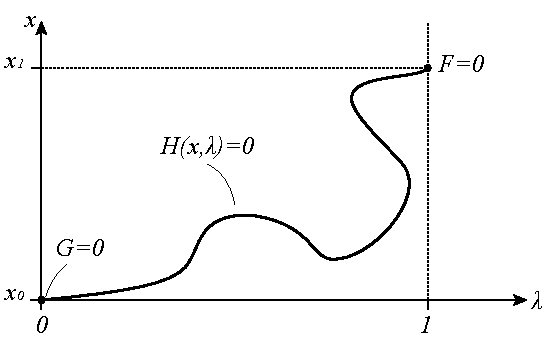
\includegraphics[scale=1.1]{FIG29.pdf}
	\caption{A homotopy path connecting the trivial solution of $G=0$ 
		to a root of $F=0$ for a single scalar equation dependent on $x$.}
	\label{fig:FIG29}
\end{figure}
The path $\mathit{\Gamma}$ depends on how $\bvec{H}$ is defined, which in turn 
is determined by the choice for $\bvec{G}$. We distinguish two general
cases of homotopy imbeddings: artificial and natural.

One typically resorts to artificial homotopies when a simple solution to problem
(\ref{eq:P1}) is generally not available. The homotopy parameter
$t$ and the simpler problem $\bvec{G}$ are then simply devices that
initialize the deformation process. In this
case, only the final point $(\bvec{x}_1,1)$ is of interest and not the path
$\mathit{\Gamma}$. A commonly used form
of artificial homotopy is the convex homotopy: 
\begin{equation}
	\bvec{H}(\bvec{x},t) = t\bvec{F}(\bvec{x})+(1-t)\bvec{G}(\bvec{x})=\bvec{0}
	\label{eq:homotopy1}
\end{equation}
Among the variety of convex homotopy functions that have been
developed, the ones most frequently used in implementations are:
\begin{itemize}
	\item{\makebox[5cm][l]{Probability one homotopy:}
		$\bvec{G}(\bvec{x})=\bvec{x}-\bvec{x}_0$}
	\cite{Chow:1978,Watson:2002}
	\item{\makebox[5cm][l]{Newton homotopy:} $\bvec{G}(\bvec{x}) =
		\bvec{F}(\bvec{x})-\bvec{F}(\bvec{x}_0)$}
	\cite{Keller:1978,Smale:1976}
	\item{\makebox[5.01cm][l]{Affine homotopy:} $\bvec{G}(\bvec{x}) =
		\bmat{F_x}_0(\bvec{x}-\bvec{x}_0)$}\ \cite{Garcia:1980,Wayburn:1987}
\end{itemize}
On the other hand, systems whose response depends on
variations of a parameter, $t$, that has physical meaning can be recast as 
natural homotopies as follows:
\begin{gather}
	\bvec{R}(\bvec{x})=0 \xrightarrow{\text{parameterization}} 
	\bvec{R}(\bvec{x},t)=0
	\label{eq:Natural}
\end{gather}

Frequently, in such cases an initial state of the system, $\bvec{R}_0$, is
easily found and the deformation process starts from there. The
process ends when one or more target states are found, which, by convention, 
correspond to $t=1$. In constrast with artificial imbeddings, the path
$\mathit{\Gamma}$ generated by Eq. (\ref{eq:Natural}) is also of interest
because all $(\bvec{x},t)\in\mathit{\Gamma}$ represent states of the
system. As an example, the residual balance equations in nonlinear mechanics, 
$\bvec{R}(\bvec{u})=\bvec{0}$, can be cast as a natural homotopy,
$\bvec{R}(\bvec{u},t)=\bvec{0}$, where $\bvec{u}$ is the displacement vector 
and $\lambda$ represents the load intensity of extern loads.

\begin{figure*}[h]
	\centering
	\subfloat[][]{{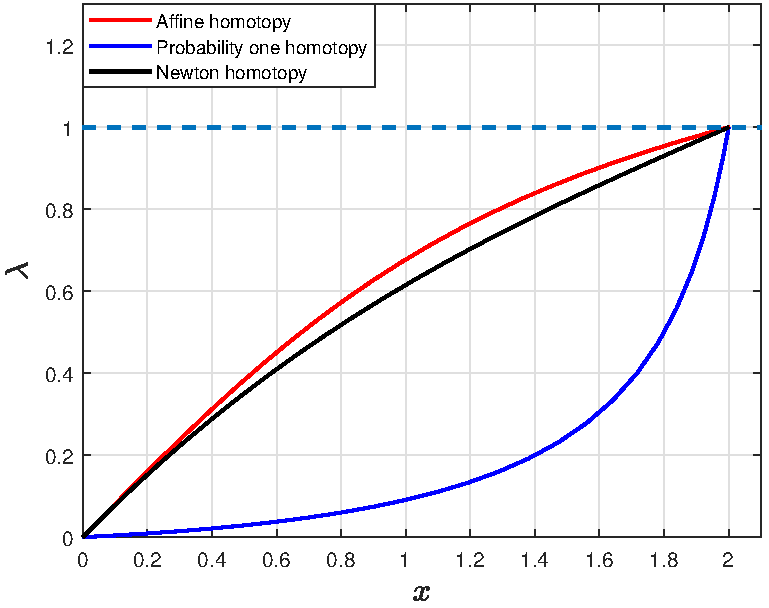
\includegraphics[width=7.0cm]{FIG30_POLYDEMO.pdf}}\label{fig:FIG30_1}}%
	\qquad
	\subfloat[][]{{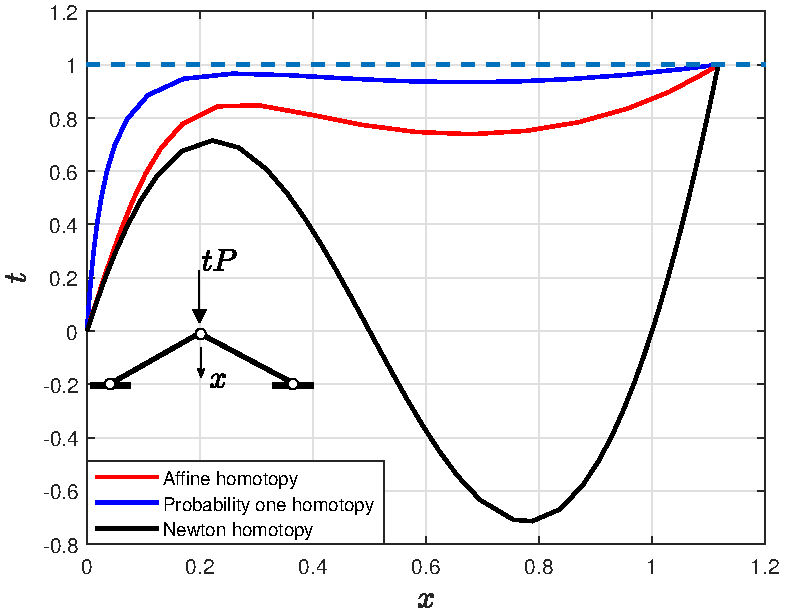
\includegraphics[width=7.15cm]{FIG30_POLYDEMO2.pdf}}\label{fig:FIG30_2}}%
	\caption{Homotopy paths for \textbf{(a)} $f(x)=x^3-6x^2+21x-26=0$, with 
		starting point
		$x_0=0$ and convergence at root $x_1=2$ when $t=1$ and 
		\textbf{(b)}
		truss, with initial state the undeformed
		configuration($x_0=0$) and target load level $P=0.03$.}%
	\label{fig:FIG30}%
\end{figure*}
\clearpage
A simple demonstration is provided in figure \ref{fig:FIG30}, where the
three artificial homotopies
mentioned above are used in two problems. In the first problem
(Fig. \ref{fig:FIG30_1}), we find a root 
of a cubic polynomial, while in the second (Fig. \ref{fig:FIG30_2}) 
we solve the 
one degree of freedom truss for target state corresponding to load $P=0.03$. 
Details for this example are taken from \cite{Rheinboldt:1981}. We see
from the truss case that while, in principle, artificial imbeddings can be 
used for systems that can be naturally parameterized, the intermediate solution
points on the path do not correspond to actual equilibrium configurations. 

%%%%%%%%%%%%%%%%%%%%%%  SECTION 1 - SUBSECTION 2  %%%%%%%%%%%%%%%%%%
\subsection{Regularity and existence of homotopy paths}\label{CH1-S1SS2}

From the discussion so far it is evident that the study of mappings
$\bvec{H}:\mathbb{R}^{n+1}\rightarrow\mathbb{R}^n$ is of primary importance. 
Consider such a mapping, $\bvec{H}(\bvec{v})$, which is at least 
of $C^k$ continuity, $k\geq 2$, with $\bvec{v}\in\mathbb{R}^{n+1}$ and $t$ 
being its $(n+1)$th component. 
For any given $\bvec{w}\in\mathbb{R}^n$, the equation 
$\bvec{H}(\bvec{v})=\bvec{w}$
represents a system of $n$ equations with $n+1$ unknowns and we designate the
subset of $\mathbb{R}^{n+1}$ satisfying this system as follows:
\begin{equation*}
	\bvec{H}^{-1}(\bvec{w}) = \{\bvec{v}\in\mathbb{R}^{n+1}\ |\ 
	\bvec{H}(\bvec{v})=\bvec{w}\}\subseteqq\mathbb{R}^{n+1}
\end{equation*}
\begin{definition}[Regular values of $\bvec{H}$]
	An element $\bvec{w}\in\mathbb{R}^n$ is a regular value of 
	$\bvec{H}:\mathbb{R}^{n+1}\rightarrow\mathbb{R}^n$ if its Jacobian,
	$\bmat{DH}$, has rank $n$ for all $\bvec{v}\in \bvec{H}^{-1}(\bvec{w})$.
	\label{def:reg}
\end{definition}
\begin{definition}[Regular points of $\bvec{H}$]
	An element $\bvec{v}\in\mathbb{R}^{n+1}$ is a regular point of
	$\bvec{H}:\mathbb{R}^{n+1}\rightarrow\mathbb{R}^n$ if its Jacobian at that 
	point is of rank $n$.
	\label{def:reqpoint}
\end{definition}
The components of the $n\times (n+1)$ Jacobian are given by $\bmat{DH}_{ij} = 
\partial H_i^{}/\partial v_j$. It follows that if $\bvec{w}$ is a regular value 
for $\bvec{H}$, then all $\bvec{v}\in\bvec{H}^{-1}(\bvec{w})$ are regular 
points. The following lemma\cite{Allgower:2003}, stated 
here without proof, plays a constitutive role in homotopy continuation theory:

\begin{lemma}
	Let $\bm{H}:\mathbb{R}^{n+1}\rightarrow\mathbb{R}^n$ be a $C^k$ map, $k\geq
	2$, and having $\bvec{0}$ as a regular value. Then, the set 
	$\bvec{H}^{-1}(\bvec{0})$ 
	is a $C^k$ 1-dimensional manifold in $\mathbb{R}^{n+1}$, comprised of
	non-intersecting components
	that are either i) homeomorphic with the unit circle $S^1$ (loops) or 
	ii) homeomorphic with the real line $\mathbb{R}$ (paths).
	\label{Lemma:manifold}
\end{lemma}
We refer to the collection of paths and loops in $\bvec{H}^{-1}(\bvec{0})$ as
(connected) components. Figure \ref{fig:FIG31} depicts a collection of such 
components for illustrative purposes. If $\bvec{0}$ is a regular value of 
$\bvec{H}$, by the
implicit function theorem, a path(loop) $\mathit{\Gamma}$ can be described as a
$C^k$ 
map $\mathit{\Gamma}:\mathbb{R}(\text{or}\ S^1)\rightarrow\mathbb{R}^{n+1}$ 
such that
$\bvec{v}=\bvec{v}(s)$. The tangent to that curve is given by
$\dot{\bvec{v}}=d\bvec{v}^{}/ds$ and is always a non-zero vector(cf.
\cite{Allgower:2003,Garcia:1980}).

\begin{figure}[t]
	
	\centering
	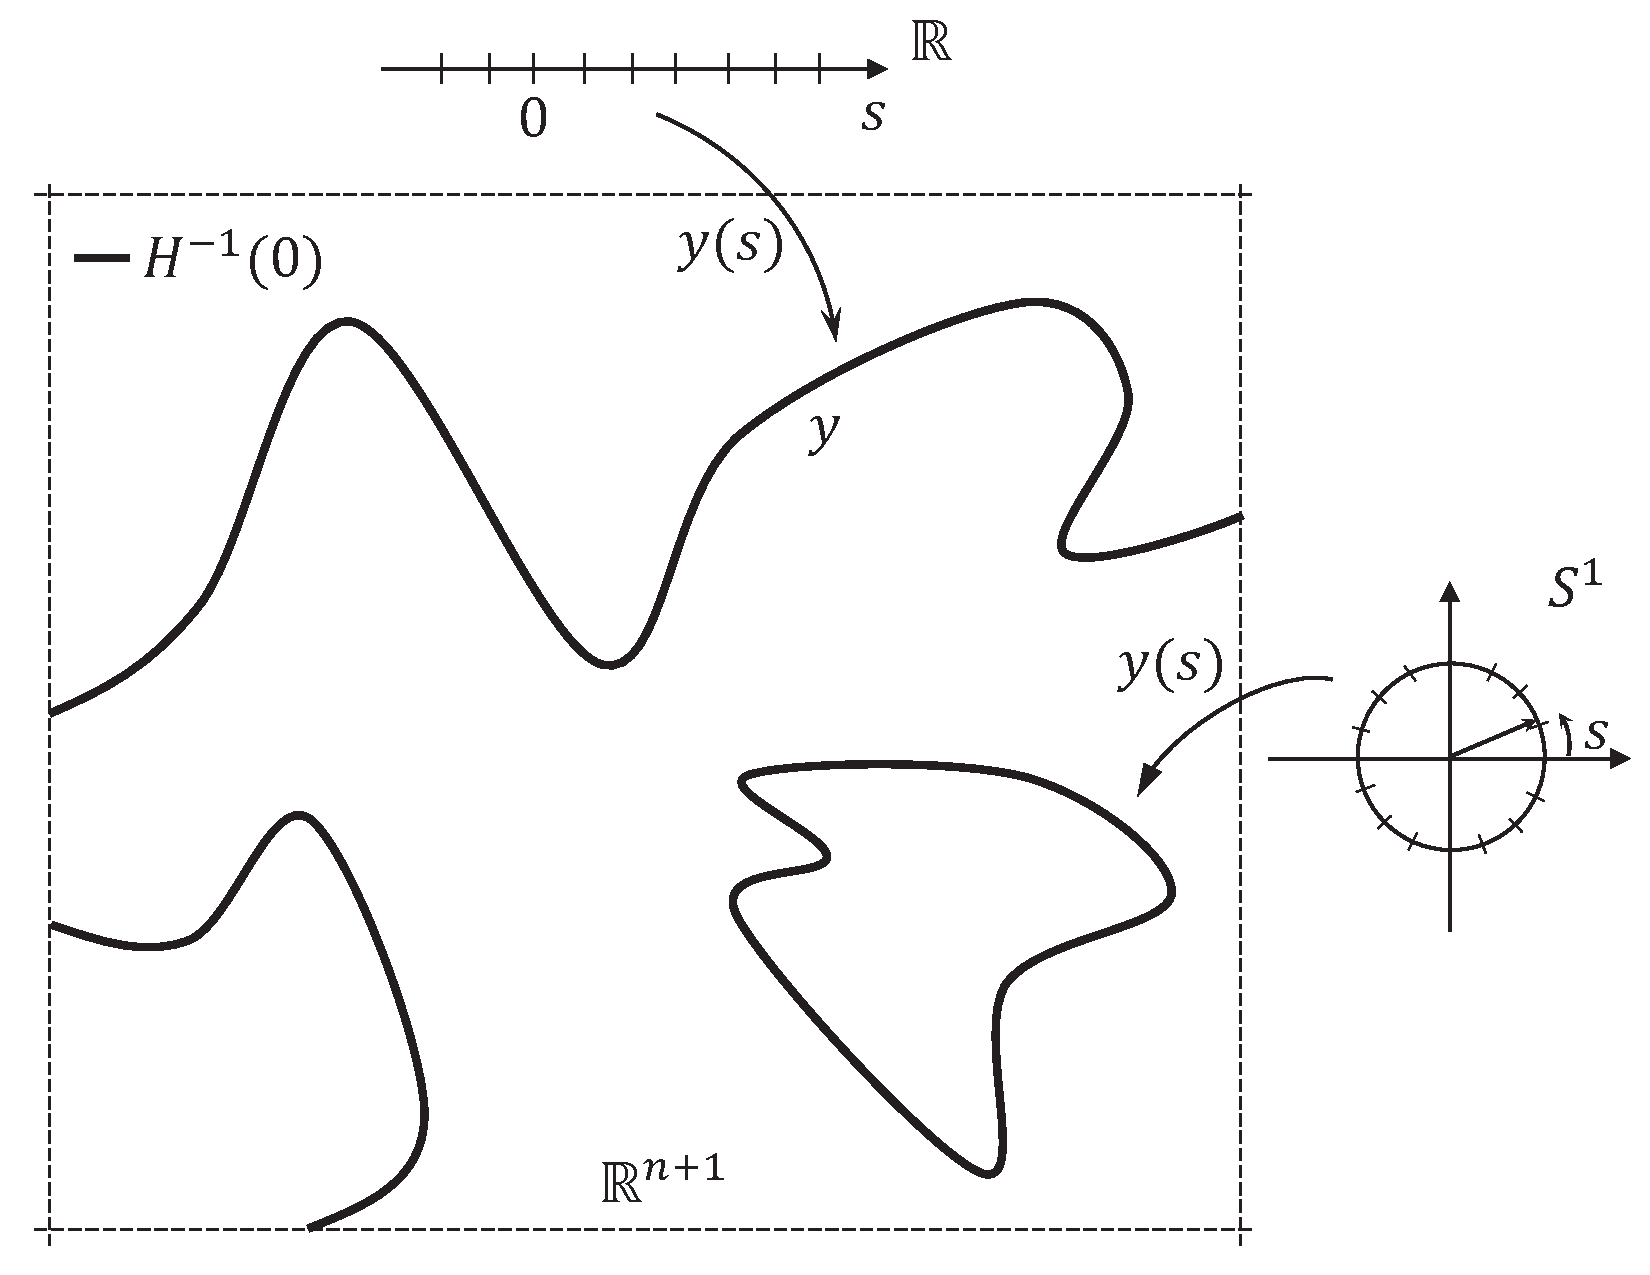
\includegraphics[scale=0.4]{FIG31_MAP.pdf}
	\caption{Components of $H^{-1}(0)$ in $\mathbb{R}^{n+1}$.}
	\label{fig:FIG31}
\end{figure}

Consider now the case of $\bvec{H}(\bvec{v})$ where the $n+1$-th component of 
$\vec{v}$ can be regarded as a special parameter of 
interest, designated as $t$. We are interested in the zero points of 
$\bvec{H}$:
\begin{equation}
	\bvec{H}(\bvec{x},t)=0
	\label{eq:GENHOM}
\end{equation}
\noindent where $\bvec{x}\in\mathbb{R}^n$, 
$t\in\mathbb{R}$. Any given initial point $(\bvec{x}_0,0)$ that satisfies Eq.
(\ref{eq:GENHOM}) sets us on a component of $\bm{H}^{-1}(\bvec{0})$ which we 
will
designate as $\mathit{\Gamma}_0$ and define as follows:
\begin{equation}
	\mathit{\Gamma}_0=\{(\bvec{x},t)\ |\ 
	\bvec{x}\in\mathbb{R}^n,\ t\in\mathbb{R},\ (\bvec{x}_0,0)\ \text{in}\ 
	\Gamma_0,\ \bvec{H}(\bvec{x}_0,0)=\bvec{0}\}
	\label{eq:PATH}
\end{equation}
In most applications we want to ensure the initial point $\bvec{x}_0$ sets us 
on 
a component $\mathit{\Gamma}_0$ which is a path, not a loop. Under the 
smoothness and regularity assumptions, the condition which guarantees that is 
for
the $n\times n$ submatrix $\bmat{DH}=\partial \bvec{H}^{}/\partial \bvec{x}$ to 
be
non-singular at $\bvec{x}_0$\cite{Garcia:1980}. More conditions are generally
required to guarantee that the path will reach $t=1$ at least once and 
depend on the particular form of $\bvec{H}$. The interested reader can refer to
\cite{Allgower:2003}, which provide proofs of existence and convergence for
various types of homotopies. In addition, it is customary to formulate
homotopies with $t\in[0,1]$. In our formulation we adhere to the
convention that a solution is reached when $t=1$. However, as is the case 
in many 
practical applications, the restriction of $t$ to lie in the unit
interval is relaxed and the parameter is allowed to take values outside of that 
range. The expectation is that more solutions will be
reached by crossing the level $t=1$ multiple times. However, it should 
be noted that homotopy theory guarantees the (global) convergence 
to one solution $(\bvec{x}_1,1)$. While certain homotopy imbeddings can find 
multiple
solutions when tracking numerically a single component
path\cite{Keller:1978,Lin:1987,Sun:1995}, it is difficult to establish
conditions that guarantee convergence to many or all solutions in
general\cite{Sun:1995}. 

%%%%%%%%%%%%%%%%%%%%%%  SECTION 1 - SUBSECTION 3  %%%%%%%%%%%%%%%%%%
\subsection{Parametric nonlinear programming}\label{CH1-S1SS3}

Our derivations follow
closely the works of Kojima \& Hirabayashi\cite{Kojima:1984}, Gfrerer et
al.\cite{Gfrerer:1983}, Gfrerer, Wacker et al.\cite{Gfrerer:1985}, Guddat et
al.\cite{Guddat:1990}.
Consider the following one-parameter optimization program:
\begin{equation}
	\hspace*{-4.5cm}\textbf{P}(t): \hspace*{3.8cm}\text{min}\{f(\bvec{x},t)\ |\
	\bvec{x}\in\Omega(t),\
	t\in\mathbb{R}\}
	\label{eq:PNLP}
\end{equation}
\noindent with
\begin{equation}
	\Omega(t)=\{\bvec{x}\in\mathbb{R}^n\ |\ h_i(\bvec{x},t)=0,\ 
	i\in\mathit{I}_h,\
	g_j(\bvec{x},t)\leq 0,\ j\in\mathit{I}_g\}
	\label{eq:ConstraintSet}
\end{equation}
\noindent where we assume that functions
$f:\mathbb{R}^{n+1}\rightarrow\mathbb{R},h_i:\mathbb{R}^{n+1}\rightarrow\mathbb{R}$
and $g_j:\mathbb{R}^{n+1}\rightarrow\mathbb{R}$  are considered to
be $C^k$, $k\geq 3$, $\mathit{I}_h=\{1,\cdots,l\}$,
$\mathit{I}_g=\{1,\cdots,p\}$ and $l\ll n$, $p\ll n$. Let
$\mathcal{L}(\bvec{x},\bvec{\lambda},\bvec{\mu},t)$ be the corresponding 
Lagrangian 
function of
problem \textbf{P}$(t)$:
\begin{equation}
	\mathcal{L}(\bvec{x},\bvec{\lambda},\bvec{\mu},t) =
	f(\bvec{x},t)+\sum_{i\in\mathit{I}_h}\lambda_ih_i(\bvec{x},t)+\sum_{j\in\mathit{I}_g}
	\mu_jg_j(\bvec{x},t)
	\label{eq:Lagrangian}
\end{equation}
\noindent where $\bvec{\lambda}\in\mathbb{R}^l$ and $\bvec{\mu}\in\mathbb{R}^p$ 
are vectors of
Lagrange multipliers, with $\bvec{\lambda}=	[\lambda_1 \ \cdots \ 
\lambda_l]^T$, 
$\bvec{\mu}=[\mu_1 \ \cdots \ \mu_p]^T$. 
Additional specifications need to be imposed on set $\Omega(t)$ in order to
derive a set of equations which will determine the solution set. Two 
conditions which we base our exposition on are the Linear Independence
Constraint Qualification (\acrshort{licq}) and the Strict Complementarity 
Condition (\acrshort{scc}). Let the index set of the active inequality 
constraints be defined as follows:
\begin{equation}
	\mathit{I}_g^a(p)=\{j\ |\ g_j(\bvec{x},t)=0,\ j\in\mathit{I}_g\}
	\label{eq:activeindex}
\end{equation}

\begin{definition}[LICQ]
	At any $\bvec{x}\in\Omega(t)$, if the gradients of the active 
	constraints 
	$\{\nabla h_i, \nabla g_j\}$, $i\in\mathit{I}_h$, $j\in\mathit{I}_g^a$, is a
	set of linearly independent vectors, then the linear independence constraint
	qualification holds at $\vec{x}$.
	\label{definition:LICQ}
\end{definition}
\begin{definition}[SCC]
	At any $\bvec{x}\in\Omega(t)$, if the Lagrange multipliers of the 
	active
	set of inequality constraints are strictly positive, $\mu_j>0\ \forall
	j\in\mathit{I}_g^a$, then the strict complementarity condition holds at
	$\bvec{x}$.
	\label{definition:SCC}
\end{definition}
Under the LICQ, SSC and the smoothness assumptions, if $\bvec{x}$ is a
minimum(maximum)
point for \textbf{P}$(t)$, then there exist unique $\bvec{\lambda}$, 
$\bvec{\mu}$
such that the point $(\bvec{x},\bvec{\lambda},\bvec{\mu},t)$ satisfies the 
so-called Karush-Kuhn-Tucker (\acrshort{kkt}) system:

\begin{subequations}
	\begin{alignat}{2}
		&\hspace{-5cm}\textbf{KKT}(t):\hspace{3.3cm}
		\nabla_{\bvec{x}}\mathcal{L}(\bvec{x},\bm{\lambda},\bm{\mu},t)& 
		&=\bvec{0}\label{eq:KKT1}\\
		&h_i(\bvec{x},t)& &=0,\quad i\in\mathit{I}_h \label{eq:KKT2}\\
		&\mu_jg_j(\bvec{x},t)& &=0\label{eq:KKT3}\\
		&\mu_j\geq 0,  g_j(\bvec{x},t)& &\leq 0,\quad 
		j\in\mathit{I}_g\label{eq:KKT4}
	\end{alignat}
	\label{eq:KKT}
\end{subequations}
The primary objective of \acrshort{pnlp} is to examine the local and global 
behavior of 
points that satisfy the \textbf{KKT}$(t)$ system (\ref{eq:KKT}). It is 
conventient to recast the \acrshort{kkt} system above into a form that contains 
only 
equalities and, thus, homotopy continuation principles can be applied. 

Let $T$ be a subdivision of the augmented Lagrangian space
$\mathbb{R}^n\times\mathbb{R}^l\times\mathbb{R}^p\times\mathbb{R}$ into cells
$\tau(\bar{\mathit{I}}_g)$, where $\tau(\bar{\mathit{I}}_g) =
\mathbb{R}^n\times\mathbb{R}^l\times\{\mu\in\mathbb{R}^p\ |\ \mu_j\geq
0,j\in\bar{\mathit{I}}_g,\ \mu_j\leq 0,
j\in\mathit{I}_g\backslash\bar{\mathit{I}}_g\}\times\mathbb{R}$ for
$\bar{\mathit{I}}_g\subset\mathit{I}_g$ and $I_g\backslash\bar{I}_g = \{j\in 
I_g\ |\ j\notin \bar{I}_g\}$. That is, the space is partitioned in cells with 
each cell identified by a particular active index set. Using an active index 
set strategy, Gfrerer et al\cite{Gfrerer:1985} showed that problem
$\textbf{P}(t)$ and, consequently, $\textbf{KKT}(t)$ can be 
replaced by an equivalent reduced system, which contains only (active) equality 
constraints\cite{Guddat:1990,Gfrerer:1985}:
\begin{equation}
	\hspace*{-0.2cm}\textbf{P}^{\tau}(t): 
	\hspace*{0.4cm}\text{min}\{f(\bvec{x},t)\ |\
	h_i(\bvec{x},t)=0,i\in I_h, g_j(\bvec{x},t)=0, 
	j\in\bar{I}_g,\bvec{x}\in\mathbb{R}^n,\ t\in\mathbb{R}\}
\end{equation}
with the corresponding Lagrangian being:
\begin{equation}
	\mathcal{L}^{\tau}(\bvec{x},\bvec{\lambda},\bvec{\mu},t) =
	f(\bvec{x},t)+\sum_{i\in\mathit{I}_h}\lambda_ih_i(\bvec{x},t)+\sum_{j\in
		\bar{I}_g}\mu_jg_j(\bvec{x},t)
	\label{eq:LagrangianREDUCED}
\end{equation}

Setting
$\bvec{z}=(\bvec{x},\bvec{\lambda},\bvec{\mu})\in\mathbb{R}^{n+l+|\bar{\mathit{I}}_g|}$,
where $|\bar{\mathit{I}}_g|\leq p$ is the cardinality of $\bar{\mathit{I}}_g$, 
the reduced \acrshort{kkt} system for program \textbf{P} is:
\begin{equation}
	\hspace{-3.4cm}\textbf{KKT}^{\tau}(t):\hspace{2.0cm}\bvec{H}_{KKT}^{\tau}(\bvec{z},t)=\begin{bmatrix}
		\nabla_{\bvec{x}}\mathcal{L}^{\tau}(\bvec{z},t)\\
		-h_i(\bvec{x},t),\ i\in I_h\\ 
		-g_j(\bvec{x},t),\ j\in \bar{I}_g
	\end{bmatrix}=\begin{bmatrix}
		\bvec{0}\\0\\ 0
	\end{bmatrix}
	\label{eq:KKTER}
\end{equation}

where $\bvec{H}_{KKT}^{\tau}(\bvec{z},t):
\mathbb{R}^{n+l+|\bar{\mathit{I}}_g|+1}\rightarrow
\mathbb{R}^{n+l+|\bar{\mathit{I}}_g|}$, that is, in each cell 
$\bvec{H}_{KKT}^{\tau}$ is of the form \ref{eq:GENHOM}.
This reformulation presupposes that i) \acrshort{licq} and \acrshort{scc} 
hold throughout and ii) that $\bvec{0}$ is a 
regular value of the reduced system $\bvec{H}_{KKT}^{\tau}$ on each cell 
$\tau(\bar{I}_g)$, which in turn leads to the following 
corollaries\cite{Kojima:1984}:
\begin{enumerate}
	\item The set $\cup_{\tau}[\bvec{H}^{\tau}_{KKT}]^{-1}(\bvec{0})$ is 
	comprised of piecewise
	continuously differentiable paths(loops) on $\mathbb{R}^{n+l+p+1}$.
	\item Each path(or loop) is $C^{k-1}$ in each$\tau(\bar{I}_g)\neq 
	\varnothing$.
	\item If a path(or loop) crosses a cell boundary between cells
	$\tau(\bar{I}^{\ 1}_g)$ and $\tau(\bar{I}_g^{\ 2})$, then sets $\bar{I}^{\ 
	1}_g$ and $\bar{I}^{\ 2}_g$ differ by only one index and the tangent vector 
	to the 
	path at the intersection is not tangent to the boundary.
\end{enumerate}

 In addition, utilizing condition 3
above, there exists\cite{Gfrerer:1985} a unique subdivision 
$\mathcal{D}=\bigcup_{q=1}^Q W^q$ 
of an interval $[\alpha,\beta]$ on the real line, such that:
\begin{itemize}
	\item	$[\alpha,\beta]=\bigcup_{q=1}^Q W^q,\ \ W^q = 
	[s_q,s_{q+1}],\ 
	\text{and}\  s_1=\alpha, s_Q=\beta,\ \ q=1,\dots,Q$.
	\item $\bar{I}_g(s)=I^q\ \text{where } \mathit{I}^q=\mathit{I}^a_g(s),
	\text{for all}\ s\ \text{in}\ (s_q,s_{q+1})$.
	\item $I^q\neq I^{q+1}$.
	\item By the implicit function theorem, there exist a $C^{k-1}$ function 
	$\bvec{\phi}(s)=(\bvec{z}(s),t(s)):W^q\rightarrow
	\mathbb{R}^{n+l+|\bar{\mathit{I}}_g|+1}$.
	\item $\bvec{\phi}(s)$ is the solution set for
	$\textbf{KKT}^{\tau}(t)$ for all $s\in W^q$.
\end{itemize}

In addition, if we require that
$\Vert \text{d}\bvec{z}^{}/\text{d}s,\text{d}t^{}/\text{d}s\Vert=1$, then $s$ 
represents the arc-length of the path(or loop). By repeating the process for 
$q=1,\dots,Q$, a $C^{k-1}$ piecewise continuous 
component $\mathit{\Gamma_0}$ can be traced numerically using appropriate 
continuation 
techniques. At a particular solution point $(\bvec{z}^*,t^*)$, 
the values of inactive constraints $g_j(\bvec{x}^*,t^*)$, $ j\in I_g\backslash 
I^q$ and the Lagrange
multipliers of the active constraints, $\mu_j$, $j\in I^q$,
are checked to ensure that complementarity slackness holds (eq.
(\ref{eq:KKT4})). Since adjacent cells differ in their respective active index
sets by only one index, violation of the complementarity slackness condition
indicates that the continuation entered cell $\tau(I^{q+1})$ and there is a
unique index, $j_k$, such that:
\begin{align*}
	g_{j_k}(\bvec{x}^*,t^*)\geq 0,\ j_k\in I_g\backslash I^q\hspace*{0.5cm} 
	&\rightarrow\quad
	I^{q+1}=I^q\cup\{j_k\},\ g_{j_k}=0\\
	&\text{OR}\\
	\mu_{j_k}\leq 0,\ j_k\in I^q \hspace*{2.1cm}&\rightarrow\quad 
	I^{q+1}=I^q\backslash\{j_k\},\
	\mu_{j_k}=0\\
\end{align*}
The collection of paths and loops of stationary points satisfying 
(\ref{eq:KKT}) is depicted in Fig. \ref{fig:FIG32}. For
further details on the relevant proofs, refer to
Gfrerer et al.\cite{Gfrerer:1985} and
the textbook by Guddat, Vasquez \& Jongen\cite{Guddat:1990}.
\begin{figure}[t]
	\centering
	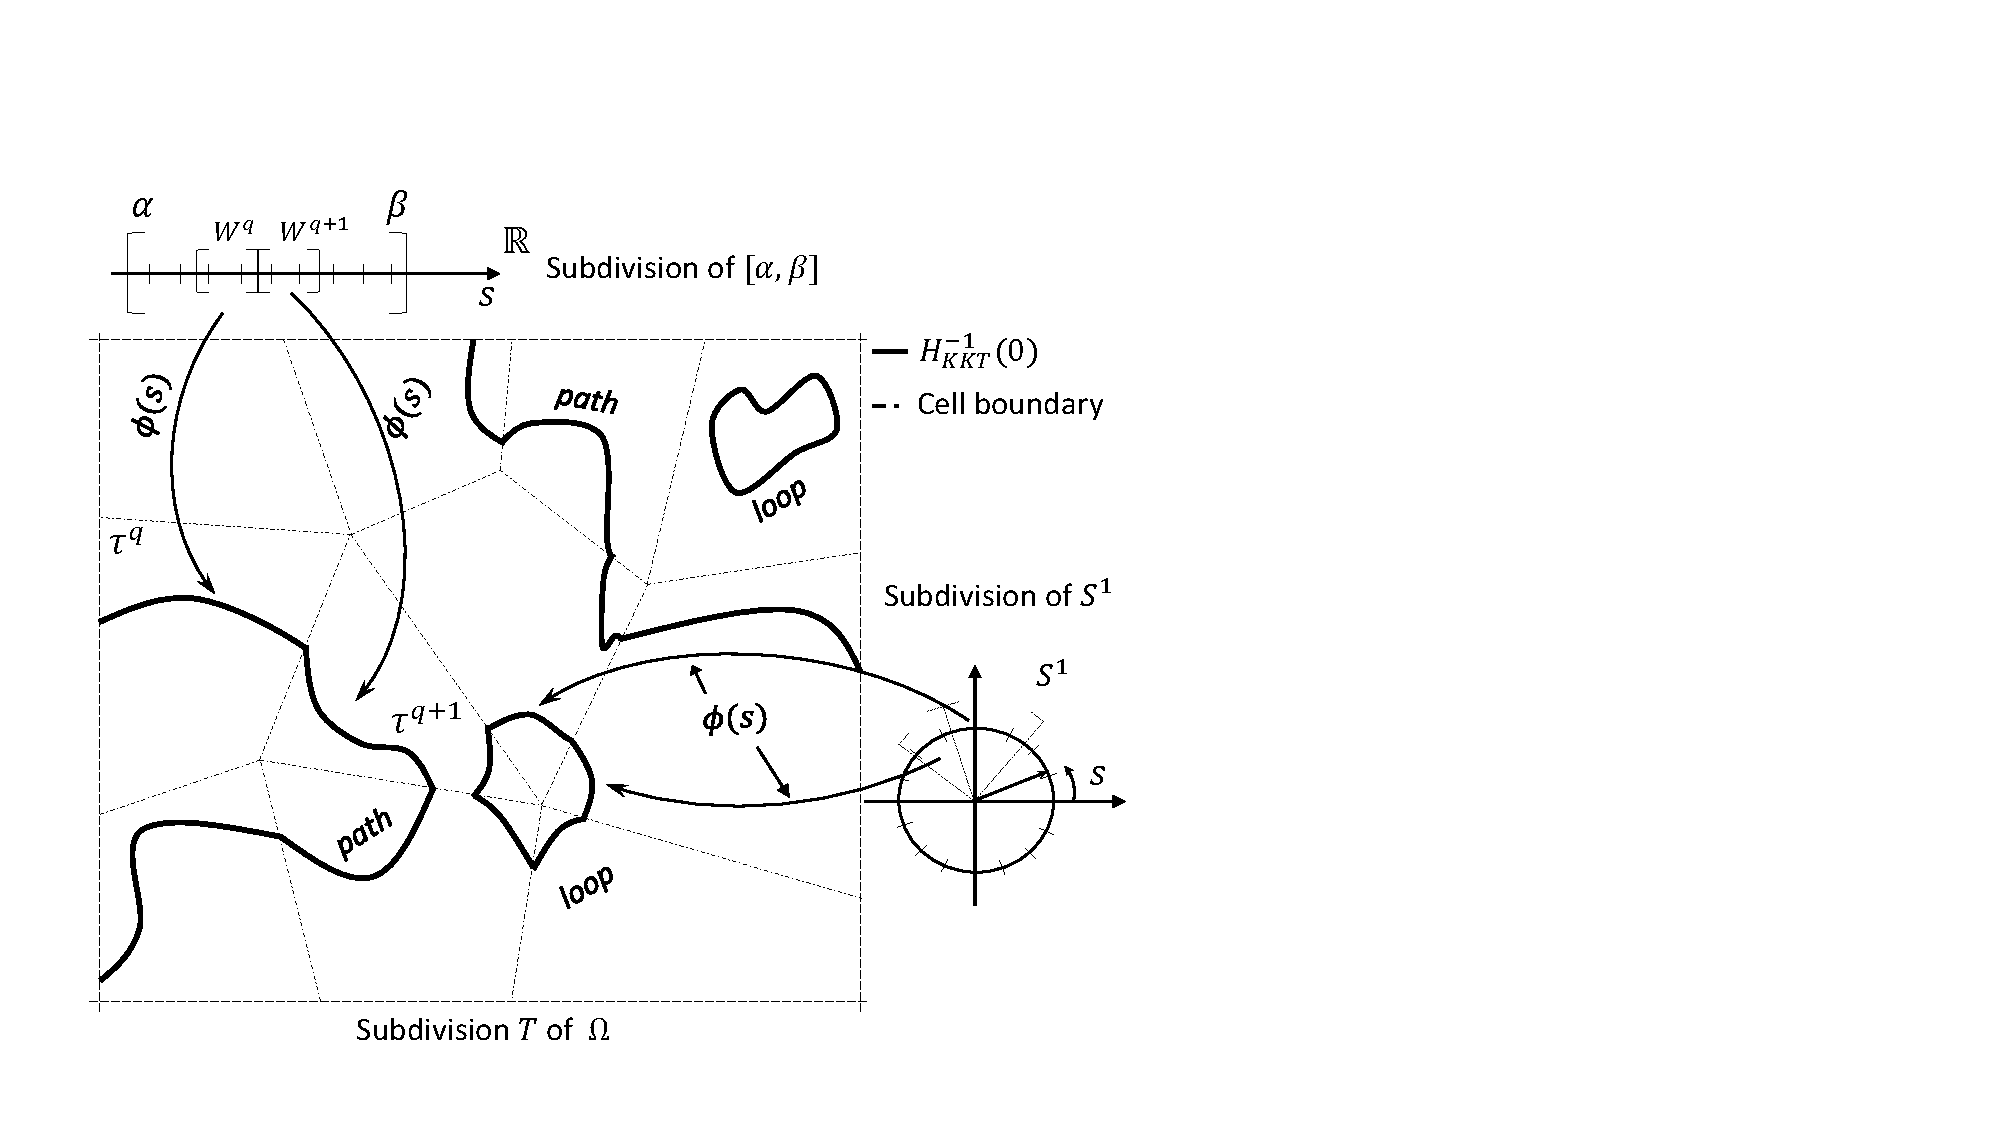
\includegraphics[scale=0.4]{FIG32_PCMAP.pdf}
	\caption{Piecewise continuously differentiable paths and loops of
		$\bm{H}_{KKT}^{-1}(\bm{0})$ in $\mathbb{R}^{n+l+p+1}$.}
	\label{fig:FIG32}
\end{figure}

%%%%%%%%%%%%%%%%%%%%%%  SECTION 1 - SUBSECTION 4  %%%%%%%%%%%%%%%%%%
\subsection{Global optimization}\label{CH1-S1SS4}

Consider the following NLP:
\begin{subequations}
	\begin{gather}
		\hspace*{-5.1cm}\textbf{P}: \hspace*{4.5cm}\text{min}\{f(\bvec{x})\ |\
		\bvec{x}\in\Omega\}\label{eq:NLP-P}\\
		\Omega=\{\bvec{x}\in\mathbb{R}^n\ |\ h_i(\bvec{x})=0,\ 
		i\in\mathit{I}_h,\
		g_j(\bvec{x})\leq 0,\ j\in\mathit{I}_g\}\label{eq:NLP-PC}
	\end{gather}
	\label{eq:NLP}
\end{subequations}
\noindent where the same assumptions hold for $f,h_i$ and $g_j$ as in 
\acrshort{pnlp} problem (\ref{eq:PNLP}). Conventional numerical tools based in 
mathematical 
analysis guarantee the convergence to a (local) minimimizer $\bvec{x}^*$ of
\textbf{P} provided that the initial guess is within the domain of convergence
for the particular method employed. By utilizing Homotopy principles, we can
convert \textbf{P} into a \acrshort{pnlp} using an appropriate imbedding. A 
numerical algorithm with global convergence properties can then be constructed, 
given that the conditions discussed previously hold. Consider the following 
one-parameter \acrshort{pnlp}:
\begin{subequations}
	\begin{gather}
		\hspace*{-3.3cm}\bm{\mathcal{P}}(t):
		\hspace*{3.1cm}\text{min}\{\mathcal{F}(\bvec{x},t)\ |\
		\bvec{x}\in\Omega(t),\ t\in[0,\ 1]\}
		\label{eq:PNLP-P}\\
		\Omega(t)=\{\bvec{x}\in\mathbb{R}^n\ |\ 
		\mathcal{H}_i(\bvec{x},t)=0,\ i\in\mathit{I}_h,\
		\mathcal{G}_j(\bvec{x},t)\leq 0,\ j\in\mathit{I}_g\} \label{eq:PNLP-PC}
	\end{gather}
	\label{eq:PNLPformat}
\end{subequations}
For $\bm{\mathcal{P}}(t)$ to be a homotopy imbedding of \textbf{P}, 
we require that:
\begin{enumerate}
	\item \acrshort{nlp} $\ \bvec{\mathcal{P}}(0)$ possesses a trivial 
	solution. 
	\item $\bvec{\mathcal{P}}(1)=$\textbf{P}
\end{enumerate}

\noindent If \textbf{P} can be naturally parameterized, then
$\bm{\mathcal{P}}(t)=$\textbf{P}$(t)$,
$\mathcal{F}(\bvec{x},t)=f(\bvec{x},t)$ and a stationary point, not necessarily
unique, of \textbf{P}$(0)$ is usually easy to compute. Artificial imbeddings can
also be employed when \textbf{P} cannot be naturally parameterized. In such
cases, a trivial stationary point for
$\bm{\mathcal{P}}(0)$ is easy to compute by construction. Below we list two 
artificial
imbeddings that are frequently used in practice:
\begin{itemize}
	\item $\mathcal{F}(\bvec{x},t) = t f(\bvec{x})+\frac{1}{2}(1-t)\Vert
	\bvec{x}-\bvec{x}_0\Vert ^2$
	\item $\mathcal{F}(\bvec{x},t) = \bvec f(\bvec{x})+\frac{1}{2}(1-\bvec)\Vert
	f(\bvec{x})-f(\bvec{x}_0)\Vert ^2$
\end{itemize}

